\documentclass{article}

\usepackage{lipsum}
\usepackage[margin=1in, left=1.5in, includefoot] {geometry}
\usepackage{amsthm}
\usepackage{listings}
\usepackage{color}
\usepackage{graphicx}
\usepackage{float}

%Code styling
\definecolor{codegreen}{rgb}{0,0.6,0}
\definecolor{codegray}{rgb}{0.5,0.5,0.5}
\definecolor{codepurple}{rgb}{0.58,0,0.82}
\definecolor{backcolour}{rgb}{0.95,0.95,0.92}
 
\lstdefinestyle{mystyle}{
    backgroundcolor=\color{backcolour},   
    commentstyle=\color{codegreen},
    keywordstyle=\color{magenta},
    numberstyle=\tiny\color{codegray},
    stringstyle=\color{codepurple},
    basicstyle=\footnotesize,
    breakatwhitespace=false,         
    breaklines=true,                 
    captionpos=b,                    
    keepspaces=true,                 
    numbers=left,                    
    numbersep=5pt,                  
    showspaces=false,                
    showstringspaces=false,
    showtabs=false,                  
    tabsize=2
}
 
\lstset{style=mystyle}

%Theorems and deffinitions
\newtheorem{theorem}{Theorem}

%Header Footer Configuration
\usepackage{fancyhdr}
\pagestyle{fancy}
\fancyfoot{}
\fancyfoot[R] {\thepage}
%
\begin{document}

%Title page
\begin{titlepage}
	\begin{center}
		\line(1,0){350} \\
		\Huge{\bfseries Data Structures and Algorithms (INFO-F413)} \\
		\line(1,0){200} \\
		[1.5cm]
		\huge{Assignment 1: Binary Space Partitions} \\
		[10cm]
	\end{center}
	
	\begin{flushright}
	\textsc{\large Joan S. Gerard S.} \\
	Computer Science Student \\
	Id Number 000471612 \\
	jgerards@ulb.ac.be\\
	8 November, 2018 \\
	
	\end{flushright}
	
\end{titlepage}

%Table of contents
\tableofcontents
\thispagestyle{empty}
\cleardoublepage

%List of figures
\listoffigures
\thispagestyle{empty}
\cleardoublepage

\setcounter{page}{1}
%Introduction
\section{Introduction}\label{sec:intro}

We have proved the following theorem during classes:

\begin{theorem}\label{the:theorem}
The expected size of the partition produced by the randomized algorithm is bounded from above by $n + 2nH_n = O(nlogn)$.
\end{theorem}

In order to demonstrate this empirically a program that creates a BSP tree was written in Python language. Such program receives as an input a text-file which contains
a set of $n$ segments $\{S_1, S_2, ..., S_n\}$, the program builds another set (size $n!$) containing the possible permutations of the original set, then
it creates a BSP tree for each permutation, it calculates its size and finally it creates four graphics:
\begin{description}
\item[$\bullet$] the set of segments in the plane.
\item[$\bullet$] the minimum and maximum size obtained after running BSP.
\item[$\bullet$] the list of the first segments chose by the BSP algorithm that produced the smallest and biggest BSP tree.
\end{description}

\section{Description of the program}\label{sec:prog_description}

In this section we will discuss some problems that were faced during the development of the program.

\subsection{Upper-Down segment division}
When the BSP algorithm choses a segment and projects a line over this segment, this line could intersect some other segments and these should be cut
into two different ones and make the upper-down division in order to keep iterating with the rest of segments until only one of them exists in the remaining plane.

When the BSP algorithm starts it will chose the first segment $S_1$ from the set of segments. $S_1$
has the coordinates $(x_1, y_1), (x_2, y_2)$ in the $(x,y)$ plan so we can easily determine the slope of the line, which we will call $m$ given by:
\begin{equation}\label{eq:1}
m = \frac{(y_2 - y_1)} {(x_2 - x_1)}
\end{equation}

Then the equation of the line is given by:
\begin{equation}\label{eq:2}
y = mx + b
\end{equation}

In order to obtain $b$ we can simply replace $(x_1,y_1)$ in equation \ref{eq:2} and we will get concrete values for $m$ and $b$. This calculation was made in the $Segment.py$ (\ref{sec:segment.py}) file by the following method:
\lstinputlisting[language=Python, firstline=16, lastline=24, caption=Line Projection Code]{Segment.py}

Note that in order to avoid division by 0 a value, epsilon, very small is added into $m$ equation.

Once we have the line projection it is easy to determine which other segments are above, below or intersected by the line projection of the chosen segment. For instance, given the segment $S_2$ with points $(x\textsubscript{21},y\textsubscript{21}),(x\textsubscript{22},y\textsubscript{22})$ and the line projection of the segment $S_1$ defined by the equation \ref{eq:2}, we want to determine the relative position of $S_2$  to the line projection of $S_1$, we simply replace $x\textsubscript{21}$ and $x\textsubscript{22}$ in equation \ref{eq:2} and we
obtain $y_1, y_2$ respectively. The result of these values can be interpreted as follows:
\begin{description}
\item[$\bullet$] If $y\textsubscript{21} > y_1$ and $y\textsubscript{22} > y_2$: the segment $S_2$ is above $S_1$.
\item[$\bullet$] If $y\textsubscript{21} < y_1$ and $y\textsubscript{22} < y_2$: the segment $S_2$ is below $S_1$.
\item[$\bullet$] If $y\textsubscript{21} > y_1$ and $y\textsubscript{22} < y_2$ (or viceversa): the segment $S_2$ intersects the line projection of $S_1$.
\item[$\bullet$] If $y\textsubscript{21} = y_1$ and $y\textsubscript{22} = y_2$: the segment $S_2$ is on the same line projection of $S_1$.
\end{description}

This is calculated by the following code in the $BSPManager.py$ (\ref{sec:BSPManager.py}) file:

\lstinputlisting[language=Python, firstline=71, lastline=86, caption=Upper-Down segment division]{BSPManager.py}

Note that the case when $S_2$ is on the same line projection of $S_1$ was not considered in this algorithm.

\subsection{Segment permutations}

Initially the program read a file which contains a set of segments, then it generates all the possible segment permutations because we want to be sure that a permutation that generates a BSP tree whose size exceeds $O(nlogn)$ does not exist. Thus, the program will generate a BSP tree for each set of segments that belongs to the permutations list. 

The file $Main.py$ (\ref{sec:Main.py}) contains the code that generates the permutations, builds the BSP tree and obtain their sizes:

\lstinputlisting[language=Python, firstline=47, lastline=63, caption=Segment Permutations Code]{Main.py}


\subsection{BSP algorithm}

The method is recursive and basically it chooses the first segment of the set, makes the upper-down division based on the line projection and calls the same algorithm for the subset of segments until there is only one segment in a cell. 
The file $BSPManager.py$ ({\ref{sec:BSPManager.py}}) contains the following code for building the BSP tree recursively given a set of segments. 

\lstinputlisting[language=Python, firstline=16, lastline=69, caption=BSP Algorigthm]{BSPManager.py}

\section{Analysis of data}

The program was tested with three different set of segments obtaining the same result.

\subsection{First case}\label{sec:first_case}
The first case corresponds to the following set of segments:

\begin{figure}[H]
	\centering
	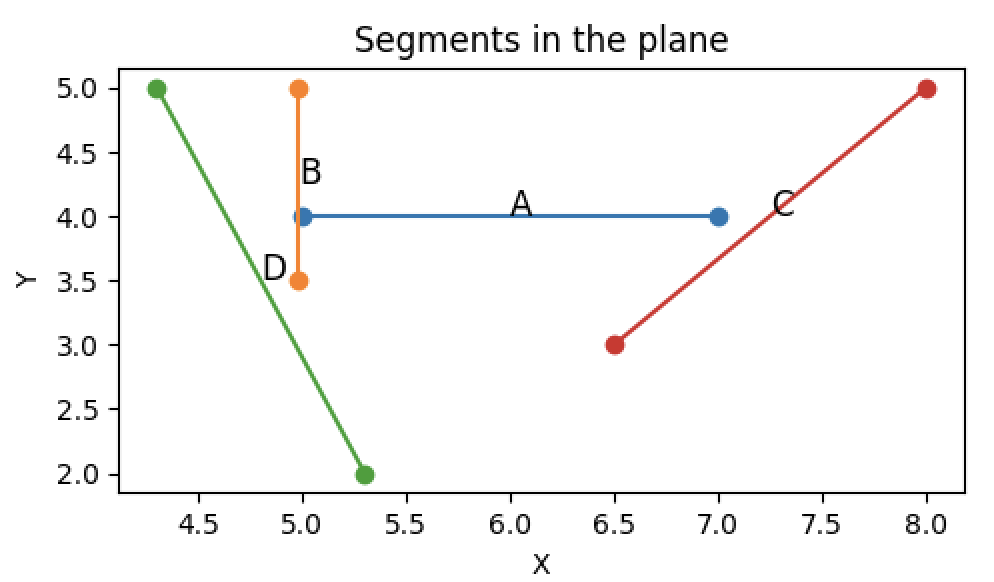
\includegraphics[height=3in]{Figure1.png}
	\caption {Set of segments from assignemnt}
	\label{fig:firstcasefig1}
\end{figure}

Figure \ref{fig:firstcasefig2} shows BSP tree size of all the possible permutations of the set of segments after running the algorithm.

Given the number of segments $(n=4)$, we have $4!$ possible combinations. Figure \ref{fig:firstcasefig2} shows that there were 3 permutations of segments that build a BSP tree with a size equals to 4, 8 of size 5, 6 of size 6, 4 of size 7 and 3 of size 8.

Figure \ref{fig:firstcasefig3} shows that permutations running BSP starting with segment C (1 permutation) or D (2 permutations) obtained a tree with size equals to 4 which corresponds to the minimum size (called minimal occurrence here).

\begin{figure}[H]
	\centering
	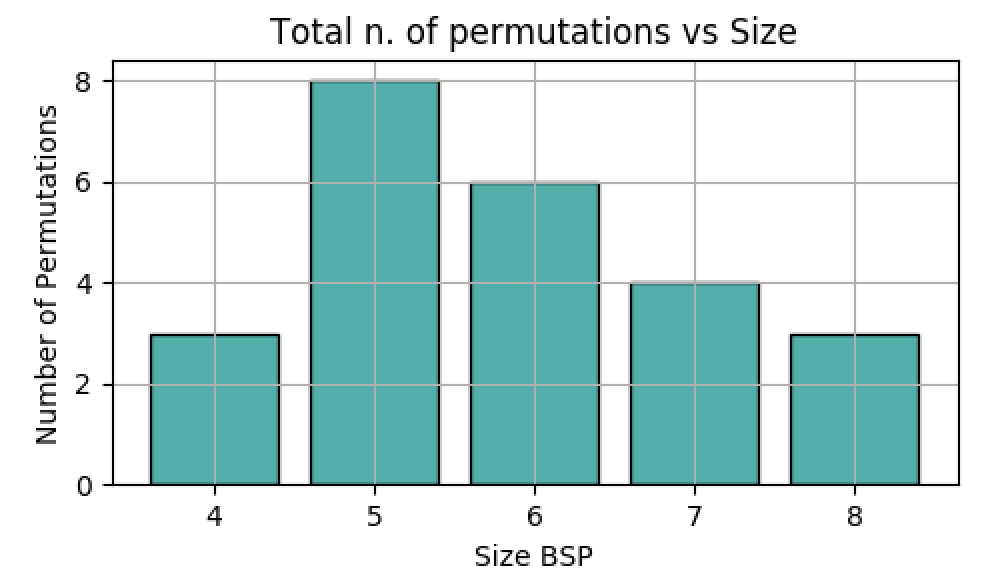
\includegraphics[height=3in]{Figure2.png}
	\caption {Permutations vs Size for first case}
	\label{fig:firstcasefig2}
\end{figure}

\begin{figure}[H]
	\centering
	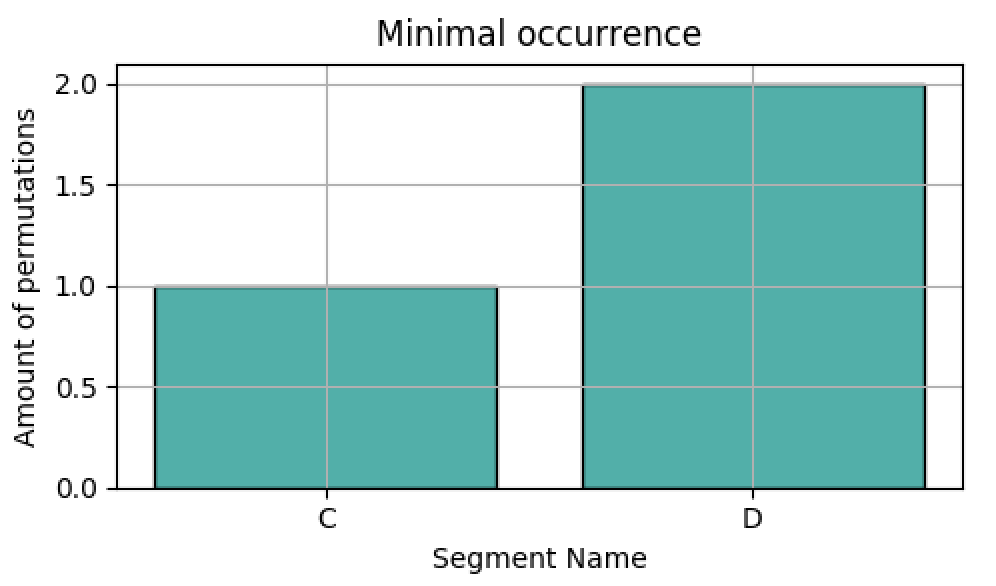
\includegraphics[height=3in]{Figure3.png}
	\caption {Best choices for first case}
	\label{fig:firstcasefig3}
\end{figure}

The figure \ref{fig:firstcasefig4} shows that those permutations that run BSP starting with segment A (3 permutations) obtained a tree with a size equals to 8 which corresponds to the maximum size (called maximal occurrence here).

\begin{figure}[H]
	\centering
	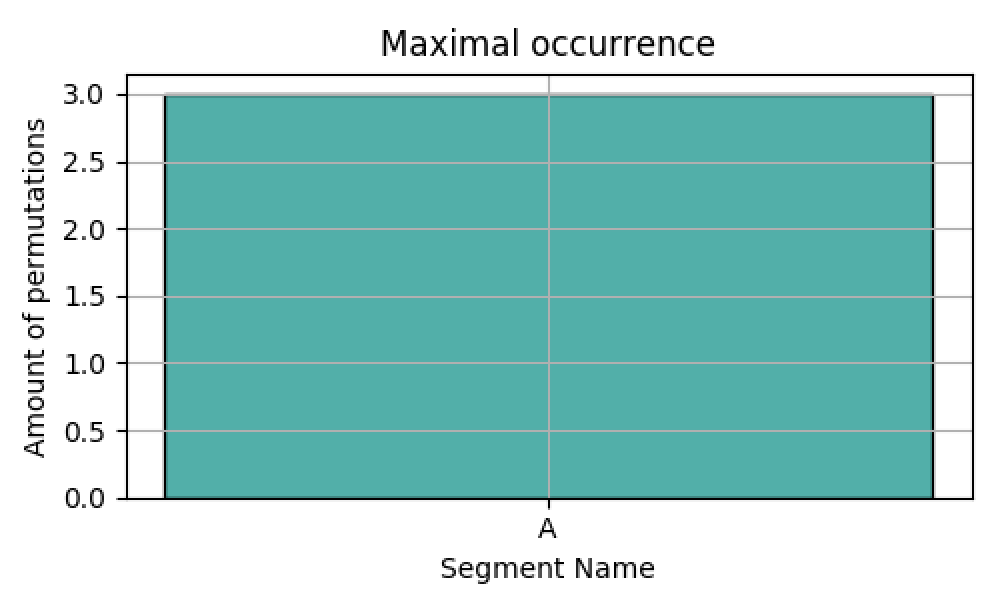
\includegraphics[height=3in]{Figure4.png}
	\caption {Worst choices for first case}
	\label{fig:firstcasefig4}
\end{figure}

The worst-case scenario generated a BSP tree of size 8 and it did not exceed the upper bound limit of $O(nlogn)$. Additionally, we also know that line projections over C and D do not intersect any other segments while the one over A intersects all others, this fact corresponds to the minimal and maximal occurrence respectively.

\subsection{Second case}

Figure \ref{fig:firstcasefig5} shows a different set of sets $(n=8)$. The maximum size for the BSP tree is 15 for this case which is again lower than the upper bound. Note also that some permutations that run BSP starting with segments B or C obtained a tree with a size equals to 8 which is the best case possible. However, those starting with A, E, G, H obtained a BSP of size 15 which is the worst case possible. Furthermore, the projection of B and C does not intersect with any other segment, this is not the case for A, E, G and H.

\subsection{Third case}

Here $n=8$ and we have some parallel segments and only one not-parallel segment.

Figure \ref{fig:firstcasefig6} shows that the maximum size for a BSP tree given the set of segments is 15 which is again lower than the upper bound. Additionally, the amount of permutations to get a BSP of size 8 is higher so the probability of choosing a permutation that generates a smaller BSP is also high. Note also that there are more permutations starting with segments B or F, which are closer to the segment A, that generates a minimum-size BSP tree. 
 
\begin{figure}[H]
	\centering
	\includegraphics[height=3.5in]{Figure5.png}
	\caption {Data analysis for the second case}
	\label{fig:firstcasefig5}
\end{figure}

\begin{figure}[H]
	\centering
	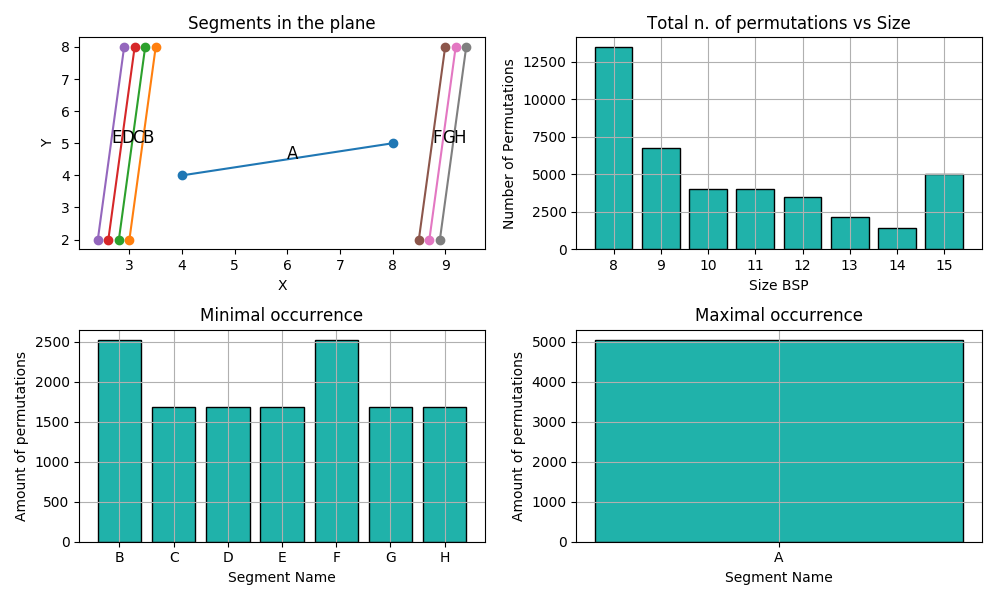
\includegraphics[height=3in]{Figure6.png}
	\caption {Data analysis for the third case}
	\label{fig:firstcasefig6}
\end{figure}


\section{Conclusions}

Based on the three cases presented above, we can see that permutations that generated the smallest binary partition for each case would be the ones starting with the segments whose line projections do not cut any other segment. 

The three cases presented on this report were chosen between other test cases and, as it was expected, none of them overpassed the upper bound limit given by theorem \ref{the:theorem}.

\cleardoublepage
\appendix
\section{Code}
Here is all the code used for this assignment.
\subsection{Node.py}
\lstinputlisting[language=Python]{Node.py}
\subsection{Line.py}
\lstinputlisting[language=Python]{Line.py}
\subsection{Segment.py}\label{sec:segment.py}
\lstinputlisting[language=Python]{Segment.py}
\subsection{BSPManager.py}\label{sec:BSPManager.py}
\lstinputlisting[language=Python]{BSPManager.py}
\subsection{Main.py}\label{sec:Main.py}
\lstinputlisting[language=Python]{Main.py}






\end{document}